\documentclass[a4paper]{article}

\usepackage{INTERSPEECH2015}

\usepackage{graphicx}
\usepackage{amssymb,amsmath,bm}
\usepackage{textcomp}
\usepackage{cleveref}

\def\vec#1{\ensuremath{\bm{{#1}}}}
\def\mat#1{\vec{#1}}

\usepackage[dvipsnames]{xcolor}
\newcommand{\TODO}[1]{{\color{red}\textbf{[TODO #1]}}}

\usepackage{enumitem}
\usepackage{booktabs}
\usepackage{multirow}
\usepackage{tipa}
\usepackage{tabularx}
\usepackage{caption}
\usepackage{subcaption}



\sloppy % better line breaks
\ninept


\title{Automatic classification of lexical stress errors for German CAPT}

%%%%%%%%%%%%%%%%%%%%%%%%%%%%%%%%%%%%%%%%%%%%%%%%%%%%%%%%%%%%%%%%%%%%%%%%%%
%% If multiple authors, uncomment and edit the lines shown below.       %%
%% Note that each line must be emphasized {\em } by itself.             %%
%% (by Stephen Martucci, author of spconf.sty).                         %%
%%%%%%%%%%%%%%%%%%%%%%%%%%%%%%%%%%%%%%%%%%%%%%%%%%%%%%%%%%%%%%%%%%%%%%%%%%
%\makeatletter
%\def\name#1{\gdef\@name{#1\\}}
%\makeatother
%\name{{\em Firstname1 Lastname1, Firstname2 Lastname2, Firstname3 Lastname3,}\\
%      {\em Firstname4 Lastname4, Firstname5 Lastname5, Firstname6 Lastname6,
%      Firstname7 Lastname7}}
%%%%%%%%%%%%%%% End of required multiple authors changes %%%%%%%%%%%%%%%%%

\makeatletter
\def\name#1{\gdef\@name{#1\\}}
\makeatother \name{{\em%
  Anjana Sofia Vakil%, J\"{u}rgen Trouvain
  %Author Name$^1$, Co-author Name$^2$
  }}

\address{%
  %$^1$Author Affiliation \\
  %$^2$Co-author Affiliation \\
  Department of Computational Linguistics \& Phonetics\\
  Saarland University, Saarbr\"{u}cken, Germany\\
  {\small \tt 
  %[%
  anjanav%
  %,trouvain%
  %]%
  @coli.uni-saarland.de}
}

%\twoauthors{Karen Sp\"{a}rck Jones.}{Department of Speech and Hearing \\
%  Brittania University, Ambridge, Voiceland \\
%  {\small \tt Karen@sh.brittania.edu} }
%  {Rose Tyler}{Department of Linguistics \\
%  University of Speechcity, Speechland \\
%  {\small \tt RTyler@ling.speech.edu} }

%
\begin{document}



  \maketitle
  %
  \begin{abstract}
  
    \TODO{Abstract (200 word limit)}
  
  	This very useful filler sentence has exactly ten different words. This very useful filler sentence has exactly ten different words. This very useful filler sentence has exactly ten different words. This very useful filler sentence has exactly ten different words. This very useful filler sentence has exactly ten different words. This very useful filler sentence has exactly ten different words. This very useful filler sentence has exactly ten different words. This very useful filler sentence has exactly ten different words. This very useful filler sentence has exactly ten different words. This very useful filler sentence has exactly ten different words. This very useful filler sentence has exactly ten different words. This very useful filler sentence has exactly ten different words. This very useful filler sentence has exactly ten different words. This very useful filler sentence has exactly ten different words. This very useful filler sentence has exactly ten different words. This very useful filler sentence has exactly ten different words. This very useful filler sentence has exactly ten different words. This very useful filler sentence has exactly ten different words. This very useful filler sentence has exactly ten different words. This very useful filler sentence has exactly ten different words. 
    
    
    
  \end{abstract}
  %
  \noindent{\bf Index Terms}: computer-assisted pronunciation training, CAPT, word prosody, German \TODO{are these OK?}


  \section{Introduction}
  
  %\cite{Vakil2015}
  
    
  %Lexical stress, the phenomenon by which a given syllable is accorded a higher level of prominence than other syllables in a given word, serves a contrastive function in some languages (e.g. German) but not others (e.g. French). Lexical stress is very important in German, and may have a large impact on the intelligibility of L2 German speech (see Section 2.4.1); however, given that lexical stress is realized extremely differently (or not at all) in French (see Section 2.3.2), the correct prosodic realization of lexical stress in German is notoriously difficult for L1 French speakers (see Section 2.3.3).
  %
%Computer-Assisted Pronunciation Training (CAPT) systems have the potential to automati- cally provide highly individualized analysis of such learner errors, as well as feedback on how to correct them, and thus to help learners achieve more intelligible pronunciation in the target language (Witt, 2012). The thesis project described here aims to advance German CAPT by creating a tool which will diagnose and offer feedback on lexical stress errors in the L2 German speech of L1 French speakers, in the hopes of ultimately helping these learners become more intelligible when speaking German.
  
  
  For adult learners of a second language (L2), the phonological system of the L2 can pose a variety of difficulties. For certain L2s, such as German or English, one important difficulty involves the accurate prosodic realization of lexical stress, i.e. the accentuation of certain syllable(s) in a given word, with the placement of stress within a word varying freely and carrying a contrastive function in such languages \cite{Cutler2005}. Lexical stress is an important part of German word prosody, and has been found to have an impact on the intelligibility of non-native German speech \cite{Hirschfeld1994}. Coping with this phenomenon in German is especially challenging for native (L1) French speakers, because lexical stress is realized very differently (or perhaps not at all) in the French language \cite{Dupoux2008,Michaux2013}.
  
  To overcome this difficulty and improve their L2 word prosody, learners typically need to have their pronunciation errors pointed out and corrected by a language instructor; unfortunately, the lack of attention typically given to pronunciation in the foreign language classroom, 
  along with other factors such as high student-to-teacher ratios,
  %coupled with the historic lack of instructor training in phonetics/phonology, 
  make this level of individualized attention not always feasible in a classroom setting \cite{Neri2002,Derwing2005,Hirschfeld2007}. Fortunately, advances in Computer-Assisted Pronunciation Training (CAPT) over recent decades have made it possible to automatically provide highly individualized analysis of learners' prosodic errors, as well as feedback on how to correct them, and thus to help learners achieve more intelligible pronunciation in the target language. However, while much research has gone into the creation and improvement of CAPT systems for English (see e.g. \cite{Eskenazi2009,Witt2012}), relatively little work has been done on the development of CAPT systems for German, especially on those targeting errors in German prosody.
  
  This paper describes work that advances the state of German CAPT by applying machine learning methods to the task of diagnosing lexical stress errors in non-native German speech, a necessary prerequisite for delivering individualized corrective feedback on such errors in a CAPT system. The paper is organized as follows: \Cref{sec:bkgd} provides background on the phenomenon of lexical stress as it is realized in German and French word prosody, motivates the creation of CAPT systems that address this error specifically, and summarizes some past work related to this topic. \Cref{sec:data} describes the manual annotation of lexical stress errors in a small corpus of L2 German speech, carried out to create labeled training and test data for the classification experiments explained in \cref{sec:method}. \Cref{sec:results} presents and analyzes the results of these experiments. Finally, \cref{sec:conc} offers some concluding remarks and outlines possible directions for future work.



	\section{Background and related work}
	\label{sec:bkgd}
	
%When there is a typological difference between some segmental or prosodic feature(s) of a language learner’s L1 compared to the target L2, there is a particular need for pronunciation training to bridge this gap. In the case of the French-German language pair, the prosodic realization of lexical stress is one feature which marks a striking difference between the languages.

Broadly speaking, lexical stress is the phenomenon of how a given syllable is accentuated within a word \cite{Cutler2005}, i.e. how a syllable is given a more prominent role such that this syllable is perceived as ``standing out'' \cite{Dogil1999}. This perceived prominence of a syllable is a function not merely of the segmental characteristics of the uttered syllable, i.e. the speech sounds it contains, but rather of its (relative) suprasegmental properties, namely:
\begin{itemize}[topsep=.5em,noitemsep]
\item duration, which equates on the perceptual level to length;
\item fundamental frequency (F0), which corresponds to perceived pitch; and 
\item \TODO{intensity (\textbf{energy?} or amplitude)}, which perceptually equates to loudness.
\end{itemize}

%As Cutler (2005) points out, different languages make use of this suprasegmental information in different ways. 
In variable-stress languages, such as German and English, 
the location of lexical stress in a word is not always predictable,
%it is not always possible to predict which syllable in a word will carry the stress, 
and therefore knowing a word requires, in part, knowing its stress pattern. This allows lexical stress to serve a contrastive function in these languages, 
%such that two words may share exactly the same sequence of phones and nevertheless be distinguished exclusively by their stress pattern, as is the case with 
e.g. distinguishing \textit{UMfahren} (to drive around) from \textit{umFAHRen} (to run over with a car) in German. 
%Because stress carries meaning thus, native speakers of such languages are sensitive to stress patterns, and readily able to perceive differences in stress. 
Furthermore, in German, misplaced stress can disrupt understanding even in cases where there is no stress-based minimal pair \cite{Hirschfeld1994}.
%, supporting the theory that speakers of free-stress languages rely to a large extent on stress information in the recognition of spoken words (Cutler, 2005).
%
However, in fixed-stress languages, stress is completely predictable, as it always falls on a certain position in the word (e.g. the final syllable), making the lexical stress pattern less crucial to the knowledge of a word than in variable-stress languages. 
%Lexical stress may not be as crucial to the knowledge of a word in these languages as in the variable-stress languages. 
Furthermore, 
%although lexical stress is realized in these languages, 
in fixed-stress languages there may be a weaker distinction between stressed and unstressed syllables.
While French has often been categorized as a fixed-stress language, given that word-final syllables are given prominence when a French word is pronounced in isolation, some argue that it may be more properly considered a language without lexical stress, in that speakers do not seem to accentuate any syllable within the word, with word-final lengthening effects explained by interactions with the realization of phrasal accent (lengthening of the final syllable in each prosodic group or phrase) \cite{Dupoux2008,Michaux2013}. 
Regardless, French has no contrastive word-level stress \cite[p.~89]{Michaux2013}, 
and in this respect differs considerably from German.
%which constitutes a significant difference between this language and a language with variable, contrastive lexical stress such as German or English.

This difference between the languages leads us to expect French learners of German to have difficulties with both perception and production of lexical stress prosody.
Although little research has been done on the nature of lexical stress errors for this particular L1-L2 pair, Hirschfeld and Trouvain \cite{Hirschfeld2007} report that such errors are commonly observed in German spoken by French natives.
Research on French speakers' perception of Spanish, another contrastive-stress language, has revealed that these speakers seem to be ``deaf'' to lexical stress, i.e. seem to have significant and lasting difficulty perceiving and remembering stress contrasts \cite{Dupoux2008}. 
With respect to production, studies of L2 Dutch have shown that French speakers, especially beginners, make systematic errors with lexical stress, exhibiting a tendency to stress the final syllable of Dutch words even when stress should be placed on the initial or medial syllable \cite{Michaux2012,Michaux2013}. Similar findings have also been reported for French learners of English \cite{Bonneau2011}.
%As a result of this difference in the sound systems of the two languages, native speakers of French may generally be expected to lack the sensitivity to stress patterns possessed by native speakers of German. Indeed, this has been borne out by research by Dupoux et al. (2008), who found that native French speakers seem to be “deaf” to lexical stress, insofar as they have significant and lasting difficulty perceiving lexical stress in Spanish, another language in which stress serves a contrastive function. This difficulty should also exist for French speakers when they are presented with German words in which the stress pattern is crucial to the word’s meaning, as in the minimal pair above.
%In addition to these difficulties with lexical stress perception, French learners of variable- stress languages such as English, German and Dutch have also been shown to have difficulties in producing stress patterns correctly. Research by Michaux et al. (2012; 2013) revealed that, as might be expected given the tendency for word- and/or phrase-final syllable prominence in French just discussed, French learners of Dutch showed a tendency to stress the final syllables of Dutch words, even when not called for by the canonical stress pattern. Indeed, with regard to German specifically, Hirschfeld and Trouvain (2007) report that lexical stress errors are commonly observed among L2 speakers with French as L1.
%In short, based on prior work on French learners of variable-stress languages, it can reason- ably be expected that L1 French learners of German as L2 will face challenges with both the perception and production of lexical stress, and that the (lack of) lexical stress system in their native language will influence their realization of lexical stress patterns in German words.	
%
	The high (anticipated) frequency of lexical stress errors in the speech of this L1-L2 group is thus one motivating factor for the creation of CAPT systems to help learners identify and correct such errors. 
	
	
	
	Another motivation behind this work's focus on lexical stress errors is the high impact such errors may have on the intelligibility of L2 German speech.
	Intelligibility, as opposed to lack of a “foreign accent,” is generally considered to be the most important goal of pronunciation training \cite{Munro1999,Neri2002,Derwing2005,Field2005,Witt2012}. The exact definition of \textit{intelligibility} is a topic of debate,
	% in the literature, as is the question of whether and how it differs from the notion of comprehensibility; here, let us follow
	but here we will follow Munro and Derwing \cite[p.~289]{Munro1999} in understanding it broadly as ``the extent to which a speaker’s message is actually understood by a listener.''
	Generally speaking, prosodic errors have often been found to have a larger impact on the perceived intelligibility of L2 speakers than segmental errors (Derwing and Munro, 2005; Hahn, 2004; Witt, 2012), and several studies have found lexical stress errors to have a particularly strong impact on intelligibility in free-stress languages like English and Dutch \cite{Cutler2005,Field2005} 
	%and German \cite{Hirschfeld1994}, 
	%Dutch, and German (Cutler, 2005; Field, 2005; Hirschfeld, 1994). Indeed, studies on perception of German L2 speech have found that among a variety of pronunciation error types, lexical stress errors have one of the most drastic impacts on intelligibility (Hirschfeld, 1994). 
	Though relatively little research has been done on how various pronunciation errors affect intelligibility in L2 German specifically, some studies suggest that 
	%prosodic errors, and 
	lexical stress errors 
	%especially, 
	may hinder intelligibility of L2 German speech more than other types of errors \cite{Hirschfeld1994,Hirschfeld2007}.
	Stress errors may also affect perception of segmental errors in the L2 learner’s speech; for example, segmental errors occurring in stressed syllables may be more noticeable than those in unstressed syllables \cite{Cutler2005,Michaux2012}. 
	%Additionally, some research indicates that prosodic errors such as lexical stress errors may have more of an impact on perceived foreign accent than segmental errors (Hahn, 2004; Witt, 2012); though it must again be stressed that intelligibility is a more important goal than lack of a foreign accent, insofar as perceived accent may contribute to difficulties being understood by native speakers, this relationship between prosody and accentedness also deserves mentioning.
	It would therefore seem that there may be a strong connection between lexical stress errors and intelligibility in L2 German speech, though more research is needed to clarify the nature of this relationship. \TODO{remove that sentence?}
	
	Though the frequency and impact of lexical stress errors in the speech of French learners of German thus constitute strong reasons to develop CAPT tools to treat such errors, in order for such systems to be viable, the feasibility of reliable automatic detection of this type of error must be demonstrated. 
	\TODO{Make rest of this par about how comparison-based diagnosis is usually used, then start new par with following sentence?}
	To our knowledge, no work has been reported on automatic classification-based diagnosis of lexical stress errors in L2 German speech, 
	%yet related work on other target languages seems encouraging. 
	but in recent years machine learning methods have been applied with apparent success to the classification of lexical stress patterns in English words. 
	Kim and Beutnagel \cite{Kim2011} experimented with various classifiers to identify stress patterns in high-quality recordings of 3- and 4-syllable English words, reporting accuracy in the 80-90\% range; in pilot experiments with low-quality recordings, however, the authors report lower accuracy: 70-80\% on L1 speech and 50-60\% on utterances by L2 speakers. 
	Similarly, Shahin et al. \cite{Shahin2012} trained Neural Networks to classify stress patterns in bisyllabic words uttered by L1 English children, 
	%with the intended application of treating childhood dysprosody, 
	and reported classification accuracy over 90\% for some stress patterns; though this work was conducted with a view to treating childhood L1 dysprosody, its relevance to our intended application of L2 CAPT is nonetheless clear.
	%
	Building on these related investigations, this paper seeks to further explore the viability of automatic classification-based detection of lexical stress errors, with a particular focus on those made by French speakers of German.
	%
	To this end, a small corpus of learner speech was manually annotated for lexical stress errors, as described in \cref{sec:data}.
	Using the resulting labeled L2 data, in addition to data from L1 German speakers, a series of supervised machine learners were trained using a variety of representations of the prosodic and other features of each word utterance (see \cref{sec:method:featuresets}, and these classifiers were evaluated with reference to the manually-produced labels of held-out test data (see \cref{sec:method:datasets}). \Cref{sec:results} presents and analyzes the results of these evaluations.
	
	
	\section{Data}
	\label{sec:data}
	
	Error-annotated speech data from German learners is a prerequisite for the supervised training and evaluation of classifiers for  lexical stress realizations in L2 German speech, yet to our knowledge no corpus of learner German with such annotation is publicly available. To fill this need, as well as to shed light on the perception of lexical stress errors in L2 German speech, a small corpus of speech by L1 French learners of German was manually annotated for such errors by native and non-native German speakers with varying levels of phonetics/phonology expertise. This section describes the data selected for annotation (\cref{sec:data:corpus}) and the method by which lexical stress realizations in this data were annotated (\cref{sec:data:annotation}), and presents an analysis of the observed inter-annotator agreement (\cref{sec:data:agreement}) and distribution of errors (\cref{sec:data:errors}) in the annotated dataset.
	
		\subsection{The IFCASL corpus of learner speech}
		\label{sec:data:corpus}		
		
		The learner speech data used in this work has been excerpted from the IFCASL corpus \cite{Trouvain2013,Fauth2014}, a collection of 
	phonetically diverse utterances in French and German spoken by both native speakers and non-native speakers with the other language as L1. This is the first known corpus of L2 speech in both directions of the French-German language pair, 
	and is thus an invaluable resource for research on pronunciation errors \TODO{between these languages}.
	
	The IFCASL corpus contains recordings of approximately 50 L1 speakers of each language reading carefully constructed sentences (and a short text) in both languages, such that both L1 and L2 speech was recorded for each speaker. Each L1 speaker group has an even gender distribution, and contains approximately 10 children (adolescents of 15-16 years of age) and 40 adults. A variety of self-reported L2 proficiency levels are also represented in the corpus: the recorded adults span levels A2 (beginner) through C1 (advanced) of the Common European Framework of Reference \TODO{footnote url}, the children levels A2 (beginner) and B1 (low intermediate).
	%As described by Fauth et al. (2014) and Trouvain et al. (2013), the IFCASL corpus contains recordings of approximately 100 speakers (50 native speakers of each of the two languages) uttering carefully constructed stimuli in both languages, such that speech in both the L1 and L2 was recorded for each speaker. In recording sessions, subjects were asked to read aloud a given sentence or longer text, and for approximately half of the L2 stimuli, subjects were allowed to listen to a recording of the text as uttered by a native speaker before recording their utterance. An even gender distribution was maintained among the speakers recorded, and both children (adolescents under 18 years of age) and adults participated in the recordings, the majority of participants being adults. While children were uniformly of beginner proficiency in their L2, adults of both beginner and advanced levels in the L2 were recorded. 
		%
	%The IFCASL corpus \citep{Trouvain2013,Fauth2014}, introduced in \cref{sec:intro:ifcasl}, contains recordings of native and non-native speech in French and German, and is thus a invaluable resource for research on pronunciation errors in this language pair, with the subset of the corpus containing L2 German speech by L1 French speakers (henceforth IFCASL-FG) being most relevant to the work reported in this thesis. As described in \cref{sec:intro:ifcasl}, speakers of varying ages, genders, and German proficiency levels are represented in the IFCASL-FG corpus; the exact number and characteristics of these speakers are presented in \cref{tab:data:speakers}.	
	
	%The subsets of the corpus most relevant to the work reported here are those containing German speech, both by L1 French speakers (henceforth IFCASL-FG) as well as by native German speakers (IFCASL-GG) \TODO{confusing sentence?}. 
	While L2 French speech is thus also captured in the IFCASL corpus, the annotation effort described here focuses exclusively on the German-language subset of the corpus. Only utterances from the sub-corpus of L2 German speech by L1 French speakers (henceforth IFCASL-FG) were manually annotated; native utterances from the L1 German sub-corpus (IFCASL-GG) were assumed to contain only correct lexical stress realizations.
	%TODO replace?
%	Details about the speakers included in the IFCASL-FG sub-corpus are given in \cref{tab:data:speakers}.
%	
%	\begin{table}
%			\centering
%			\caption[Speakers in the annotated dataset]{\TODO{remove?} Number of speakers in the portion of the IFCASL-FG corpus annotated for lexical stress, in terms of speakers' age, gender, and proficiency level \cite{Fauth2014}.}
%			\begin{tabular}{lrrrrr}
%			\toprule
%			\multirow{2}{*}{Age/gender}	&	\multicolumn{4}{c}{Proficiency level} &\multirow{2}{*}{\textbf{Totals}}\\
%			\cmidrule(lr){2-5}
%		& A2	&	B1	&	B2	&	C1	&		\\
%			\midrule
%Boy (male, 15-16 yrs.)	&	11	&	0	&	0	&	0	&	\textbf{11}	\\
%Girl (female, 15-16)&	1	&	1	&	0	&	0	&	\textbf{2}	\\
%Man	(male, 18-30) &	7	&	4	&	3	&	7	&	\textbf{21}	\\
%Woman	 (female, 18-30)&	5	&	5	&	3	&	9	&	\textbf{22}	\\
%			%\midrule
%\textbf{Totals}	&	\textbf{24}	&	\textbf{10}	&	\textbf{6}	&	\textbf{16}	&	\textbf{56}	\\
%			\bottomrule
%			\end{tabular}
%			\label{tab:data:speakers}
%		\end{table}
	
	
		
	The subset of IFCASL-FG selected for manual error annotation, (henceforth simply “the dataset”) consists of utterances of twelve bisyllabic word types (see \cref{tab:words}), each of which has primary stress on the initial syllable. 
	%These characteristics were chosen deliberately: the selected words are bisyllabic 
	Only bisyllabic words were selected to simplify comparison between stressed and unstressed syllables, and only initial-stress words because this is the stress pattern which native (L1) French speakers are expected to have the most difficulty producing in German, given the phenomenon of final lengthening in French (see \cref{sec:bkgd}).
	%Though previous work on lexical stress errors in L2 speech has often dealt with words uttered in isolation (e.g. Bonneau and Colotte, 2011), this work deals with word utterances extracted from longer utterances of complete sentences; as Neri et al. (2002, p. 6) point out, for relevance to real communication it is important that CAPT systems address connected speech. The word’s position in the carrier phrase/sentence was not taken into account; although it could be hypothesized that phrase position would have an effect on lexical stress realization by native French speakers, given the phenomenon of phrasal accent in French (see Section 2.3.2), Michaux and Caspers (2013) found no effect of phrase position on French speakers’ realization of words in Dutch. Given the similarities in the lexical stress systems of Dutch and German with respect to French, no such phrase-level effect is therefore expected here, though investigation of the effect of phrase or sentence position on stress realization could be an interesting direction for future work.
	

	
\begin{table}
		\centering
		\caption[Word types annotated for lexical stress errors]{%
		%The twelve bisyllabic initial-stress 
		Word types selected from the IFCASL corpus for lexical stress error annotation. 
		%The orthographic form (text) of each word type is presented in the leftmost column, followed by its canonical pronunciation (e.g. as found in a pronunciation dictionary). 
		Canonical pronunciations for each word type are given in IPA notation.
		% SAMPA notation (\url{http://www.phon.ucl.ac.uk/home/sampa}), with phonemes separated by a space and syllables separated by a period (\texttt{.}); canonical lexical stress is not marked, as all of the listed word types have primary stress on the initial syllable. 
		%Parts of speech are abbreviated as n. (noun), v. (verb) and pro. (pronoun). 
		The rightmost column lists the number of tokens (utterances) of each word type in the annotated dataset.
		}
%		\begin{tabular}{llll}
%		Flagge & Ringen & Tschechen & halten \\
%		M\"{o}rder & Tatort & Fr\"{u}hling & fliegen \\
%		Pollen & manche & E-mail & tragen \\
%		\end{tabular}
		
		{\renewcommand{\arraystretch}{1.1}
		\begin{tabularx}{\columnwidth}{lXXXl}
		%\begin{tabular}{llllc}
		\toprule
		
		Word & 
		%Canonical \linebreak 
		Pronun-ciation & 
		%Pron. &
		Part of speech & 
		%P.O.S. &
		English meaning & 
		%Recording condition \TODO{remove?}& 
		Tokens\\%\linebreak annotated\\
		
		\midrule
		E-mail		
			&	\textipa{/"i:.meIl/} %\texttt{i:~.~m eI l} 		
			&	noun
			&	e-mail %&	SR 	
			&	56	\\
			
		Flagge		
			&	\textipa{/"fla.g@/} %\texttt{f l a~.~g @} 		
			&	noun 
			&	 flag %&	SH	
			&	55	\\
			
		fliegen		
			&	\textipa{/"fli:.g\s{n}/} %\texttt{f l i:~.~g =n} 	
			&	verb 
			&	to fly %&	SR		
			& 56	\\
			
		Frühling	
			&	\textipa{/"fry:.lIN/}	%\texttt{f r y:~.~l I N} 		
			& noun	
			&	spring \newline (season) %&	SR		
			&	56	\\
			
		halten		
			&	\textipa{/"hal.t\s{n}/}	%\texttt{h a l~.~t =n}		
			&	verb 
			&	to hold %&	SR 	
			&	56	\\
			
		manche	
			&	\textipa{/"man.\c{c}@/}	%\texttt{m a n~.~C @} 		
			&	pronoun 
			&	some %& 	SR 	
			&	56	\\
			
		Mörder		
			&	\textipa{/"m\oe5.d5/}	%\texttt{m 96~.~d 6}		
			&	noun 
			&	murderer %&	SR 	
			&	56	\\
			
		Pollen		
			&	\textipa{/"pO.l@n/}	%\texttt{p O~.~l @ n} 		
			&	noun 
			&	pollen %&	SR 	
			& 	55	\\
			
		Ringen		
			&	\textipa{/"KIN.@n/}	%\texttt{r I N~.~@ n}		
			&	noun 
			&	rings %&	SH	
			&	55	\\
			
		Tatort		
			&	\textipa{/"ta:t.PO5t/}	%\texttt{t a:~t~.~?~O6 t}	
			&	noun 
			&	crime scene %& 	SR 	
			&	56	\\
			
		tragen		
			&	\textipa{/"tKa:.g\s{n}/}	%\texttt{t r a:~.~g =n} 	
			&	verb 
			&	to wear %&	SH	
			&	55	\\
			
		Tschechen	
			& \textipa{/"tSE.\c{c}\s{n}/}	%\texttt{tS E~.~C =n}	
			& noun	
			&	Czechs	%&	SR		
			& 56	\\
			
		\bottomrule
		\end{tabularx}
		}
		\label{tab:words}
	\end{table}
	
	In addition to the recordings themselves, the IFCASL corpus contains phone- and word-level segmentations of each utterance, produced automatically by forced alignment with the corresponding text prompts \cite{Fauth2014}. Although the corpus also contains manual corrections of these segmentations, the work reported here relies exclusively on the automatically-generated segmentations to more accurately represent the conditions of a real-world CAPT system, which would not have recourse to manual verification of the phone or word boundaries identified by the aligner. 
	As the IFCASL corpus does not include syllable-level segmentations, boundaries between syllables were determined automatically from the phone- and word-level segmentations of each utterance.
	
	Using the automatic segmentations, tokens (utterances) of each selected word type were extracted from the recorded segmentations automatically using Praat\TODO{footnote url}; counts of the available tokens for each word type are listed in \cref{tab:words}. 
	The dataset annotated for lexical stress errors comprises 668 word tokens in total. Five tokens had to be excluded from the dataset, as sentence-level disfluencies (e.g. false starts or repetitions of phrases) prevented accurate automatic extraction of the word utterance; a fully-fledged CAPT system would need to deal with such disfluencies automatically, e.g. with a pre-processing step  which detects disfluencies and prompts the learner to re-record their utterance if needed 
	(see e.g. %Bonneau2012
	\cite{Orosanu2012}).
	%To compile the dataset, utterances (tokens) of each word as produced by over 50 L2 speakers were extracted from the recordings automatically with Praat\TODO{footnote url}, using extraction times (start and end points of word utterances) taken from the word-level segmentation of each sentence utterance automatically obtained by forced alignment (see Section 4.1). Table 3.2 lists the exact number of tokens available for each word type. In total, 668 word tokens were annotated for lexical stress errors. Five tokens had to be excluded from the data, as disfluencies in the sentence utterance (e.g. false starts or repetitions of the target word) prevented the automatic extraction of the word utterance from the sentence as a whole. In a fully-fledged student-facing CAPT system, such disfluencies would need to be dealt with accordingly, e.g. by means of a pre-processing step which analyzes the student’s utterance for possible disfluencies and compensates for any that are detected by, for example, prompting the student to re-record their utterance. However, detecting disfluencies in speech, especially non-native speech, is a challenging problem under active research (see Section 2.2.1), and the development of a disfluency-aware system is outside the scope of this thesis project; therefore, this work presupposes that no disfluencies exist in the student’s utterance, and the handful of disfluent tokens have been excluded from the dataset described here.
		
		\subsection{Annotation method}
		\label{sec:data:annotation}	
		
		The annotation task consisted of assigning one of the following labels to each word token (utterance) in the dataset described in the previous section:
		\begin{itemize}
	\item{[correct]: the speaker clearly stressed the correct (initial) syllable}
	\item{[incorrect]: the speaker clearly stressed the incorrect (final) syllable}
	\item{[none]: the speaker did not clearly stress either syllable, 
	%i.e. did not audibly differentiate stressed and unstressed syllables, 
	or the annotator was unable to determine which syllable was stressed}
	\item{[bad\_nsylls]: the speaker pronounced an incorrect number of syllables (e.g. inserted an extra syllable), making it impossible to judge if stress was realized correctly}
	\item{[bad\_audio]: a problem with the audio file (e.g. noise or inaccurate segmentation) interfered with the annotator's ability to judge the stress realization}
	 \end{itemize}
	 
	 Annotation was performed using a graphical tool scripted in Praat. This tool displayed the given word's text, and allowed the annotator to listen to the given word utterance and the sentence utterance from which it was extracted as many times as they wished. Once they had reached a judgment about the lexical stress realization of the utterance, the annotator had to click one of five buttons, corresponding to the possible labels, to record their judgment.
	 A single annotation session consisted of annotating all 55-56 tokens of each of three word types, and lasted approximately 15 minutes.
	 %Annotation proceeded by means of a graphical tool scripted in Praat (Boersma and Weenink, 2014), the main interface of which is shown in Figure 3.1. At the top, a word’s text is displayed, along with the IFCASL corpus ID number of the speaker whose utterance of that word will be annotated (this number is only relevant for the annotator insofar as changes in its value inform the annotator that the speaker is changing from utterance to utterance). The recording of the word is played once automatically; the annotator may then choose to click one of the green buttons to play the word again, or play the recording of the entire sentence, as many times as they wish. Once the annotator has judged the accuracy of the lexical stress realization in this utterance, they log that judgment by clicking one of the gray buttons. The annotator is then automatically advanced to the next utterance, with the counts in the lower right corner tracking their progress towards the total number of tokens to be annotated.
		
		A total of 15 annotators participated, varying with respect to their L1 and level of phonetics/phonology expertise. 
		The native languages represented included German (12 annotators), English (2), and Hebrew (1); the L1 English and Hebrew speakers all speak German as \TODO{a} L2. 
		In terms of expertise, the annotators were broadly categorized as \textit{experts} (professional phonetics/phonology researchers), \textit{intermediates} (university students enrolled in an experimental phonology course), or \textit{novices} (those with negligible phonetics/phonology training or experience annotating speech data). Among the 15 annotators, there were two experts, 10 intermediates, and three novices. 		
		%
		%A total of 15 annotators participated in the annotation of this dataset, each of whom is listed in Table 3.3 (by an arbitrary identifier, to preserve anonymity). As Table 3.3 shows, the annotators varied with respect to their native language, as well as with respect to their level of expertise in phonetics/phonology/linguistic annotation.
		%
		%Of the 15 annotators, the majority (12) are native German speakers, and three are non-native (L2) speakers: two are native speakers of American English, and one is a native Hebrew speaker. The L2 German speakers all have some knowledge of German as L2, though the exact German proficiency levels of these annotators are unknown.
		%
		%In terms of expertise, the annotators can broadly be categorized into three groups:
%• expert annotators are professional researchers with a thorough understanding of phonetics/phonology and extensive experience in annotating speech data
%• intermediate annotators are university students enrolled in an experimental phonology course, and have some training in phonetics/phonology and/or experience annotating speech data
%• novice annotators have negligible training in phonetics/phonology and little, if any, experience annotating speech data
%As shown in Table 3.3, the majority of annotators (10 out of 15) fall into the intermediate group; two annotators can be considered expert, and there are three novice annotators.


		
		
		Each annotator was assigned three word types to annotate in a single session, with the exception of one who annotated six word types over two sessions. 
		%Table 3.3 lists the word types assigned to each annotator, along with the number of tokens labeled for each type. Some judgments by annotators D and G had to be excluded from the analysis due to technical problems; the token counts for each annotator in Table 3.3 reflect only their usable judgments.
		Assignments ensured that each word token was annotated by at least two native German speakers, and to maximize the amount of overlap between annotators in order to obtain as many pairwise measures of annotator agreement as possible 
		(see \cref{sec:data:agreement}).
		%(see Section 3.4 for a discussion of inter-annotator agreement); Table 3.4 lists the number of annotators for each word type.
		
		%A single annotation session consisted of annotating all tokens of three word types, and lasted approximately 15 minutes. As mentioned in Section 3.2 above, each annotator participated in one session, with the exception of annotator K who participated in two sessions (separated by several days) and annotated a total of six word types.

	
		%The lexical stress error annotations collected in this manner for each token (utterance) in the dataset enable two important contributions of this thesis, described in the following sections. First, the multiple annotations for each token from different annotators permit an analysis of inter-annotator agreement with regard to the identification of lexical stress errors; Section 3.4 presents this analysis, along with statistics on the relative frequencies with which the five labels were selected by annotators from the different L1 and expertise groups described in Section 3.2. Secondly, and perhaps more importantly, the errors identified by these annotators in the data extracted from the IFCASL corpus enable an analysis of the frequency of lexical stress errors in the speech of L1 French learners of German as L2; this is the subject of Section 3.6.
		
		
		\subsection{Inter-annotator agreement}
		\label{sec:data:agreement}		
		
		Any evaluation of an automatic error detection system, including that described in this work, should be performed with an understanding of the difficulty of the error-detection task for human listeners. To obtain a clearer picture of this task, we therefore conducted an analysis of the inter-annotator agreement observed in the annotations collected as described in the previous section. If human annotators often disagree about whether a given L2 utterance contains a lexical stress error, this may indicate that the task is a difficult one, thus encouraging a more lenient evaluation of an automatic error-detection system. However, if humans are generally in strong agreement, this may reflect a lower level of difficulty, and give reason to judge the performance of an automatic system by a higher standard. 
		%To create a useful CAPT system for lexical stress errors in L2 German, i.e. to automatically detect whether a student has made a lexical stress error in a given utterance, it is helpful to have an understanding of the difficulty of the error-detection task, not only for machines but for humans. It is therefore useful to analyze the collected stress accuracy judgments in terms of inter-annotator agreement, in order to gain insight into the nature of the challenge this task presents. If it is uncommon for human annotators to agree about whether a given lexical stress realization is correct or incorrect, this may indicate that identifying lexical stress errors is a challenging task, and one which an automatic system should also be expected to have difficulty with. If, on the other hand, human annotators are generally in strong agreement, this may reflect a lower level of difficulty, and give reason to judge the performance of an automatic system by a higher standard.
		
		
		For 268 of the 668 utterances annotated, i.e. approximately 40\% of the dataset, annotators were unanimous in their label assignments; for the other 400 utterances (60\%), at least one annotator chose a different label than the other(s) who annotated the same utterance.
		To make sense of these differences, agreement in label assignments was calculated for each pair of annotators who overlapped, i.e. labeled any of the same tokens. 
		Pairwise agreement was quantified in terms of percentage agreement (i.e. the number of tokens to which the two annotators assigned the same label, divided by the total number of tokens they both annotated), and Cohen's Kappa ($\kappa$) statistic \cite{Cohen1960}.
		To obtain an overall measure of inter-annotator agreement for the entire annotated dataset, the agreement between each pair of overlapping annotators was calculated, and the minimum, median, mean, and maximum values over all pairwise comparisons were computed; these values are given in \cref{tab:agreement:overall}.
		
		\begin{table}
			\centering
			\caption{Overall pairwise agreement between annotators}
			\begin{tabular}{lrr}
			\toprule
				&	\% Agreement	&	Cohen's $\kappa$	\\
			\midrule
Mean		&	54.92\%	&	0.23	\\
Maximum	&	83.93\%	&	0.61	\\
Median		&	55.36\%	&	0.26	\\
Minimum	&	23.21\%	&	-0.01	\\
			\bottomrule
			\end{tabular}						
			\label{tab:agreement:overall}
		\end{table}
		
		This simple analysis reveals a few interesting observations. First, the mean and median percentage agreement values near 55\% indicate that annotators seem to agree about the accuracy of lexical stress realizations just slightly more than they disagree, and the mean and median $\kappa$ values near 0.25 characterizes the overall agreement as ``fair'' in the Landis and Koch schema \cite{Landis1977}. However, the minimum and maximum $\kappa$ values reveal that agreement between different pairs of annotators ranges from ``poor'' to ``substantial'' \cite{Landis1977}, as also reflected in the correspondingly large gap between the minimum and maximum percentage agreement observed.
	%Turning to the $\kappa$ values, given that $\kappa = 0$ represents agreement purely by chance while $k = 1$ represents perfect, meaningful agreement, the fact that the mean and median $\kappa$ values between annotators are somewhere near 0.25 indicates that the agreement observed between annotators is closer to what would be expected simply by chance than to agreement that would indicate highly reliable annotations, and signifies ``fair'' agreement between annotators according to the thresholds proposed by \textcite{Landis1977}. Examination of the minimum and maximum values reveals that while some pairs of annotators seem to exhibit ``substantial'' agreement, indicating reasonably reliable judgments, other pairs have ``poor'' agreement; in one case, with 23.21\% agreement, the annotators seem to be closer to perfect disagreement than perfect agreement, and the corresponding $\kappa$ being below zero indicates that they agreed even (slightly) less than one would expect if they were merely labeling utterances randomly. 
		On the whole, then, it appears that inter-annotator agreement in this error annotation task is relatively low, though there seems to be considerable variation between individual annotators. This may simply signal that (some of) the particular annotators participating in this study are not very reliable in their judgments of lexical stress accuracy, but it may also indicate that diagnosing errors in L1 French speakers' realizations of lexical stress in German is a difficult task, even for humans.
		%; this notion will be revisited in \cref{sec:diag:classification}. 
	
	

		
		
		
		%To put the agreement values reported in this section in context, it is worthwhile to compare them with those obtained in recent work by \textcite{Michaux2013} on L2 Dutch speech by L1 French speakers. In this study, three expert annotators were asked to indicate which syllable they perceived as stressed in Dutch word utterances by the L1 French speakers. Two of the annotators were L1 Dutch speakers, the other an L1 French speaker who was nevertheless ``highly proficient'' in Dutch (p.~90). The authors report an average $\kappa$ of 0.71 between annotators, representing ``substantial'' agreement in the schema of \textcite{Landis1977}, and a much higher value than those observed in the present work. One plausible explanation for this difference may be the fact that while the three annotators participating in the \textcite{Michaux2013} study were all ``phonetically trained'' (p.~90), i.e. experts (see \cref{sec:lexstress:annotators}), the annotation project described here collected judgments from a larger number of annotators, and only two of the 15 participating annotators had extensive phonetic training. The relationship between annotator expertise and inter-annotator agreement is explored further in \cref{sec:agreement:expert}. 
		
			
		
		
		\subsection{Error distribution}
		\label{sec:data:errors}
		
		Though the comparison of the (potentially different) labels assigned to each word utterance by different annotators is interesting, a single ``gold-standard'' label for each utterance ultimately had to be determined, as a representation of the ground truth with which to train and evaluate the automatic error classifier(s) \TODO{rewrite that sentence}.
		In some cases, assigning a gold-standard label was trivial, e.g. when all or a majority of annotators agreed. However, in other cases a choice had to be made between competing candidate labels. 
		%In these cases the gold-standard label was chosen via a rule-based procedure which 
		\TODO{The decision-making procedure} prioritized experts' judgments, favored certain  judgments ([correct] or [incorrect]) over uncertain ([none]), and gave learners the benefit of the doubt when annotators disagreed as to whether the utterance was [correct] or [incorrect].
	
		\TODO{Add exact token/\% numbers, so \cref{tab:errors} can go}
		To shed further light on the error classification task, the overall distribution of lexical stress errors in the annotated dataset 
		was analyzed with reference to the gold-standard labels thus determined.
		As seen in \cref{tab:errors} and illustrated in \cref{fig:errors}, 
		%Evidently, 
		most (63.77\%) of learners' lexical stress productions were judged to be correct; in other words, almost two-thirds of the time, learners clearly stressed the correct (initial) syllable in the uttered word.
		However, learners also seemed to make mistakes regularly, with 29.64\% of their word utterances labeled [incorrect] and another 5.24\% labeled [none].
		%However, incorrect productions (productions in which the learner clearly stressed the incorrect syllable) and productions in which the learner did not clearly stress either syllable (corresponding to the [none] label, as described in \cref{sec:lexstress:method}), also occurred regularly: 29.64\% of the productions were judged incorrect and 5.24\% were labeled [none]. 	
		If we consider both [incorrect] and [none] utterances as types of lexical stress errors, then errors were observed in just over one-third of utterances. %(34.88\%) of the  utterances annotated. 
		%
		This considerable proportion of errors seems to confirm the expectation (mentioned in \cref{sec:bkgd}) that French learners of German frequently make lexical stress errors.
		
		\begin{table}
			\centering
			\caption{Overall frequency of lexical stress errors in the annotated data \TODO{remove}}
			\begin{tabular}{lrr}
			\toprule
			Label & Tokens & \% of corpus \\
			\midrule
			correct	& 426	& 63.77\% \\
			incorrect &	198	& 29.64\% \\
			none	 &35 &	5.24\% \\
			bad\_nsylls	& 8	& 1.20\% \\
			bad\_audio	& 1	& 0.15\%\\
			\midrule
			%\addlinespace
			Total & 668 & 100\%\\
			\bottomrule
			\end{tabular}
			\label{tab:errors}
		\end{table}
		
		\begin{figure}
			\centering
			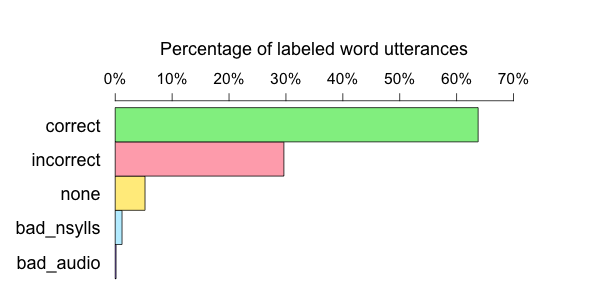
\includegraphics[width=\columnwidth]{../../img/plots/overallJudgments-axisTop-noLabels}
			\caption{Overall distribution of lexical stress errors in the annotated data}
			\label{fig:errors}
		\end{figure}
	
	
	
	
	\section{Method}
	\label{sec:method}
	
	As mentioned in \cref{sec:bkgd}, the classification-based approach to identifying lexical stress errors has not been sufficiently explored in CAPT research, especially research on CAPT for German. 
	By way of a preliminary investigation of the feasibility of this type of error diagnosis, a series of classification experiments were conducted in an effort to determine:
	\TODO{
	\begin{itemize}%[topsep=-.5em]
	 \item{how accurately lexical errors can be automatically classified, in comparison to the accuracy of human listeners in identifying such errors,}
	 \item{which of the prosodic features discussed in \cref{sec:diag:prosody} are most useful for classification, and}
	 \item{whether a classification-based approach can lead to reasonably accurate diagnosis for words or speakers not seen in the training data.}
	 \end{itemize}
	}
	% The remainder of this section describes these experiments, and \cref{sec:results} presents their findings. 
	
	 
	 The WEKA machine learning toolkit\TODO{footnote URL} was used to train and evaluate classifiers for these experiments. In this work, only simple Classification And Regression Tree (CART) classifiers \TODO{Breiman1984?} were used.
	 Many other classification algorithms are implemented in WEKA, some of which could  conceivably offer better performance; here, CARTs were chosen for their simple training process and their ease of interpretation by humans. 
	 In future work (see \cref{sec:conc}), it would be interesting to compare different classification algorithms to see if other classifiers are more effective for this type of data, along the lines of the experiments by Kim and Beutnagel \cite{Kim2011}.

		\TODO{paraphrase the below}

		For each relevant configuration (see \cref{sec:method:featuresets,sec:method:datasets}), a CART is trained to classify utterances as belonging to one of the five label categories described in \cref{sec:data:annotation}. 
		In practice, however, these trees classify every utterance as either [correct] or [incorrect], neglecting [none] and the other labels due to their comparatively low frequency in the data. 
		Overall classification accuracy on the annotated sub-corpus was assessed by using held-out portions of the annotated data as test sets, and performing cross-evaluation on multiple train/test splits of the data. The features and divisions of data used in each experiment are described in the sections below.
	
	
	    \subsection{Feature sets}
	    \label{sec:method:featuresets}
	    
	    To represent the lexical stress prosody of an utterance, the automatically-determined word, syllable, and phone segmentations were used to isolate relevant segments of the speech signal, and extract features related to the three acoustic properties mentioned in \cref{sec:bkgd} above: duration, fundamental frequency (F0), and energy. To account for inter-speaker variability, e.g. the fact that some speakers may have a faster speech rate or higher F0 than others, relative rather than absolute features were used. This section explains how these prosodic features, listed in \cref{tab:prosfeatures}, were selected and computed.
	    %The automatically-determined word, syllable, and phone boundaries obtained as described in the previous section enable the CAPT tool to locate and analyze segments of the speech signal relevant to the realization of lexical stress. This section describes the features by which the system analyzes the lexical stress prosody of an utterance, be it the utterance of a learner or of a native speaker. These features relate to the three acoustic properties (and by extension their perceptual correlates) described in Section 2.3, namely duration (timing), fundamental frequency (pitch), and intensity (loudness). The relative utility of these features in automatically diagnosing lexical stress errors is discussed further in Section 4.4.
	    
	    Research on the phonetic realization of lexical stress has often indicated that duration may be the most important, if not the only, acoustic correlate of this phenomenon in German, with the duration of stressed syllables being relatively long in comparison with unstressed syllables \cite{Dogil1999}. 
	    Therefore, features representing duration were computed, simply by noting the relative durations of relevant segments in the phone- and syllable-level segmentations. Following Bonneau and Colotte~\cite{Bonneau2011}, we take into account the durations of entire syllables, as well as of their nuclei (vowels or syllabic consonants such as /\textipa{\s{n}}/), as described in \cref{tab:durfeatures}.
	    %Analysis of duration (timing) is extremely important for detecting stress patterns; indeed, some research indicates that syllable duration may be the most important, if not the only acoustic correlate of lexical stress in German (e.g. \cite{Dogil1999}). Duration analysis therefore figures prominently in the analysis and assessment of learners' lexical stress in this work. 
	    %
	    %Given the word-, syllable- and phone-level segmentations of an utterance (see \cref{sec:diag:segmentation}), the extraction of duration features for that utterance is trivial, as it consists simply of noting the duration of each relevant segment. % in the appropriate segmentation. Following \textcite{Bonneau2011}, duration analysis in this work takes into account the  duration of each syllable in the word to be analyzed, and of the vowels at the nucleus of each syllable. 	To account for inter-speaker variability, e.g. the fact that some speakers may have an overall slower or faster speech rate than others, relative rather than absolute durations are used. The list of duration features computed for each word utterance is given in \cref{tab:durationfeatures}, along with the values computed for each feature from the sample utterances shown in \cref{fig:featuresexample}.
	    %
	    
	   After duration, the next best acoustic correlate of lexical stress appears to be F0 \cite{Dogil1999}, so F0 features were also computed (see \cref{tab:f0features}).
	    The F0 contour of a given utterance is estimated using the pitch detection functionality of the speech-processing program JSnoori\TODO{footnote URL} \cite{DiMartino1999}, which uses a spectral comb method to compute pitch points from each FFT spectrum extracted from the relevant signal segment; here spectra were extracted using Hamming windows 32-milliseconds long, offset by 8 ms. Points are computed in Hz, then converted to semitones before features are computed. Features only take into account non-zero points, i.e. those corresponding to voiced segments.
	    Though work on assessing L2 English stress has often made the assumption that stressed syllables should have higher F0 than unstressed ones (e.g. \cite{Bonneau2011}), in German stressed syllables may also have a lower F0 than other syllable(s) in the word \cite[p.~267]{Cutler2005}. Therefore, as \cref{tab:f0features} shows, our features capture not only the maximum F0 in each syllable (nucleus), but also the minimum and range (maximum$-$minimum).
	    %Much of the work on assessing non-native lexical stress has been conducted with English as the L2, and thus often makes the assumption that a stressed syllable should have a higher F0 than unstressed syllables (Bonneau and Colotte, 2011). In German, the F0 of a stressed syllable also tends to differ from the surrounding contour, but the difference may be positive (the stressed syllable has a higher pitch than surrounding syllables) or negative (lower pitch) (Cutler, 2005, p. 267). Therefore, the computed features capture not only the F0 maximum of each syllable, but also the minimum and range (difference between maximum and minimum).
	    
	    Past research indicates that a signal's energy (intensity) also reflects lexical stress patterns, though to a lesser extent than duration or F0 \cite{Dogil1999,Cutler2005}.
	   % Research on lexical stress prosody has generally indicated that intensity is the least important of the three features, i.e. corresponds least closely to lexical stress patterns (Cutler, 2005). Indeed, existing lexical stress assessment tools may not take intensity into account, as was the case with the prosodic diagnosis functionality of JSnoori at the start of this thesis project. However, intensity can nonetheless have an impact on the perception of lexical stress, especially in combination with pitch or duration, or both (ibid.); Therefore, in addition to duration and fundamental frequency, JSnoori’s learner speech analysis module was modified to take intensity (energy)2 into account.
	   Therefore, energy contours of syllables and their nuclei were also computed, again using JSnoori, which calculates the total amount of energy at frequencies from 0 to 8000 Hz in FFT spectra extracted from the signal (using Hamming windows 20 ms. long offset by 4 ms). Energy values below 60 decibels are not counted toward the total, as these are assumed to correspond to ambient or non-speech noise. Using these contours, we compute features taking into account the mean and maximum energy in the relevant segments, as shown in \cref{tab:enerfeatures}.
	    
	    \begin{table}
		\centering
		%\caption[Features used for duration analysis]{Features used for duration analysis, and their values for the sample utterances of ``Flagge'' in \cref{fig:featuresexample}. 
		\caption{%
		Prosodic features.
		%Features used to represent lexical stress prosody. 
		S0 refers to the word's first syllable, S1 to the second syllable; similarly, V0 and V1 refer to the nucleus (vowel) of the first and second syllable, respectively.
		}
		
		\begin{subtable}{\columnwidth}
		\centering
		\caption{Duration (DUR) feature set}
		 \begin{tabularx}{\columnwidth}{lX}%{lXcc}
		\toprule
		Feature name & Description \\
		%\multirow{2}{*}{Feature name} 
		%& \multirow{2}{*}{Description}
		%& \multicolumn{2}{c}{Value} \\
		%&		 &  (a) G		& (b) F \\
		\midrule
		REL-S-DUR 	
			& \mbox{Duration of S1}$/$\mbox{duration of S0}
			%& 	0.50		& 	1.00	
			\\
		REL-V-DUR 		
			& \mbox{Duration of V1}$/$\mbox{duration of V0}
			%& 	0.56		& 	1.71	
			\\
		\bottomrule	
		\end{tabularx}
		\label{tab:durfeatures}
		\end{subtable}
		
		\vspace{1em}
		
		\begin{subtable}{\columnwidth}
		\caption{Fundamental frequency (F0) feature set}
		{\renewcommand{\arraystretch}{1.25}%
		\begin{tabularx}{\columnwidth}{lX}%{lXrr}
		\toprule
		Feature name & Description \\
		\midrule
		REL-S-F0-MEAN 
			& Mean F0 in S1$/$ mean F0 in S0 \\
		REL-S-F0-MAX 
			& Maximum F0 in S1$/$ max. F0 in S0 \\
		REL-S-F0-MIN 
			& Minimum F0 %($>$0) 
				in S1$/$ min. F0 in S0 \\
		REL-S-F0-RANGE
			& F0 Range (max. F0$-$min. F0) in S1$/$ F0 range in S0 \\
		
		REL-V-F0-MEAN 
			& Mean F0 in V1$/$mean F0 in V0 \\
		REL-V-F0-MAX 
			& Max. F0 in V1$/$max. F0 in V0 \\
		REL-V-F0-MIN 
			& Min. F0 in V1$/$min. F0 in V0 \\
		REL-V-F0-RANGE 
			& F0 Range in V1$/$F0 range in V0 \\
		
%		F0-MAX-INDEX	
%			& $\begin{cases}
%					0 & \text{if max. F0 in S0}>\text{max. F0 in S1}\\
%					1 & \text{otherwise}\\
%				\end{cases}$ \\
%		F0-MIN-INDEX	
%			& $\begin{cases}
%					0 & \text{if min. F0 in S0}<\text{min. F0 in S1}\\
%					1 & \text{otherwise}\\
%				\end{cases}$ \\
%		F0-MAXRANGE-INDEX	
%			& $\begin{cases}
%					0 & \text{if F0 range in S0}>\text{F0 range in S1}\\
%					1 & \text{otherwise}\\
%				\end{cases}$ \\
		
		\bottomrule
		\end{tabularx}
		} % end arraystretch
		\label{tab:f0features}
		\end{subtable}
		
		
		\vspace{1em}
		
		\begin{subtable}{\columnwidth}
		\caption{Energy (ENER) feature set}
		\begin{tabularx}{\columnwidth}{Xl}%{lXrr}
		\toprule
		Feature name & Description \\
		\midrule
		REL-S-ENER-MEAN 
			& Mean energy in S1$/$S0 mean en.
			%&  0.39 & 0.38 
			\\
			
		REL-S-ENER-MAX 
			& Maximum en. in S1$/$S0 max. en.
			%&  0.52 & 0.45
			\\
			
		REL-V-ENER-MEAN 
			& Mean en. in V1$/$mean en. in V0
			%&  0.43 	& 0.43
			\\
			
		REL-V-ENER-MAX 
			& Max. en. in S1$/$max. en. in S0
			%&  0.53 	& 0.61
			\\
			
%		ENER-MAX-INDEX 
%			& $\begin{cases}
%					0 & \text{if S0 max. en.}>\text{S1 max. en.}\\
%					1 & \text{otherwise}\\
%				\end{cases}$
%			& 0	& 0\\
			
		\bottomrule
		\end{tabularx}
		\label{tab:enerfeatures}
		\end{subtable}
		
		
		\label{tab:prosfeatures}
		\end{table}
		
		 Using different combinations of these feature sets, a series of experiments was conducted to determine which features give the best accuracy in the error-classification task. Establishing which features perform best not only enables the creation of the most accurate classification-based error diagnosis system possible, but may also clarify whether and how strongly these acoustic properties correspond with perceived lexical stress errors in L2 German.
		 In addition to the prosodic features (\cref{tab:prosfeatures}), features representing the word type uttered and characteristics of the speaker (see \cref{tab:spkrfeatures}) were also included in the experiments, to ascertain whether including such features could improve performance.
		The results of these feature experiments are presented in \cref{sec:results:features}.
		
		\begin{table}
			\centering
			\caption{Speaker/word features}
			\begin{tabularx}{\columnwidth}{lX}
			%\begin{tabular}{ll}
			\toprule
			Feature name & Description \\
			\midrule
			WD %WORD 
				& Word type uttered (e.g. \textit{Tatort}) \\
			LVL % LEVEL 
				& Speaker's L2 German skill level \newline (A2$|$B1$|$B2$|$C1)\\
			GEN %GENDER 
				& Speaker's age/gender category \newline (Girl$|$Boy$|$Woman$|$Man)\\
%			LVL+GEN & LEVEL, GENDER \\
%			WD+LVL & WORD, LEVEL \\
%			WD+GEN & WORD, GENDER \\
%			WD+SPKR & WORD, LEVEL, GENDER \\
			\bottomrule
			\end{tabularx}
			\label{tab:spkrfeatures}		
		\end{table}
	    
	    
	    \subsection{Datasets for training and testing}
	    \label{sec:method:datasets}

		%In addition to the L2 utterances and their gold-standard labels from the annotated dataset (see Section 3.5), the corresponding L1 utterances of the selected word types from the the IFCASL-GG corpus were also included in training data, with each native utterance labeled as [correct] based on the assumption that native speakers always realize lexical stress correctly.


		
		%A 10-fold cross-validation was performed on the entire set of available training data, i.e. the utterances of 12 German word types produced by L1 French speakers which had been annotated for lexical stress errors as described in Chapter 3, along with the utterances of these word types by native German speakers, labeled as correct. As the goal of error diagnosis by classification in the CAPT context is to classify non-native speech, including native utterances in the test data was not appropriate; therefore, for each of the 10 folds of the cross-validation, one tenth of the non-native utterances were randomly selected to be held out as the test data set, and the other nine-tenths were combined with the native utterances to create the training data set.
		%To evaluate feature performance, classifiers were trained using various subsets of the com- plete feature set, which are listed in Table 4.4. For each of these feature combinations, classifiers were trained on each of the 10 training sets created as just described, and tested on the corresponding test set. The averages of each of the aforementioned evaluation metrics (see Section 4.4.1) across all 10 folds are reported.
		
		
		%one motivation for a classification-based approach to error diagnosis is that the abstraction from concrete reference utterances afforded by such a method can theoretically enable the diagnosis of errors in new word types without requiring additional recordings of native speakers pronouncing these words; to assess the feasibility of diagnosing utterances of new words, the classifier’s performance on words not seen in the training data must be evaluated and compared with the performance observed on seen words, with the hypothesis that the former will be better than the latter. Furthermore, in order for a CAPT tool to be useful in practice, it must be able to diagnose the speech of a learner from their very first time using the system. In the experiments reported above, it is possible that the training data’s inclusion of other utterances by the speaker in question resulted in higher performance than would be observed if such utterances were not available as training instances, so the classifier’s performance on unseen speakers must be compared to the performance reported above, once again with the hypothesis that the classifier will perform more poorly on unseen test data. To test these hypotheses, another series of experiments was carried out using different configurations of testing and training data sets.
		%To create training and testing data for experiments with utterances from unseen speakers, the entire set of labeled non-native utterances (see Section 4.4.1) was divided into 56 subsets, each containing all utterances from one of the 56 unique non-native speakers. Using a classifier trained on the native German utterances as well as those of the other 55 speakers, performance on each of these 56 test sets was evaluated. To investigate whether adding features related to speaker or word characteristics is more helpful than prosodic features alone when diagnosing unseen speakers’ errors, a comparison was made between classifiers trained using several combinations of the best features from the experiments described in Section 4.4.2 above. The results of the unseen-speaker experiments, and the different feature sets used for training, are given in Table 4.7.
		%To evaluate classification performance on unseen word types, the non-native utterances annotated for lexical stress (see Section 4.4.1) were divided by their word type, resulting in twelve different data sets to be used for testing. To construct the training set for each test set, utterances of the target word type were removed from the complete set of native German utterances, and the resulting set of 11 word types uttered by L1 German speakers was combined with the utterances of those 11 word types by L2 speakers. Given the improvement in performance observed with the inclusion of speaker-related features (see Section 4.4.2), along with the apparent interplay between such features and the prosodic feature set (such that overall performance improved when all prosodic features were included, not just the best-performing prosodic features of duration and F0), classifiers were trained using a few different combinations of features, to ascertain how these features affect performance when the test data consists of unseen words. It might be the case that including information about the speaker, i.e. their age/gender and proficiency level, may be more helpful when there are no training instances available for the given word type.

	\section{Results}
	\label{sec:results}
	
		\subsection{Feature performance}
		\label{sec:results:features}		
		
		\subsection{Performance on unknown words}
		\subsection{Performance on unknown speakers}
	
	%\section{Alternative error diagnosis methods}


	%\section{Discussion}

	\section{Conclusions and future work}
	\label{sec:conc}
	
	%\section{Future work}
	%\label{sec:future}



  %TODO \section{Acknowledgements}
  



  %\newpage
  \eightpt
  \bibliographystyle{IEEEtran-nourl}

  \bibliography{../../library.bib}
  %\bibliography{slaterefs.bib}

%  \begin{thebibliography}{9}
%    \bibitem[1]{Davis80-COP}
%      S.\ B.\ Davis and P.\ Mermelstein,
%      ``Comparison of parametric representation for monosyllabic word recognition in continuously spoken sentences,''
%      \textit{IEEE Transactions on Acoustics, Speech and Signal Processing}, vol.~28, no.~4, pp.~357--366, 1980.
%    \bibitem[2]{Rabiner89-ATO}
%      L.\ R.\ Rabiner,
%      ``A tutorial on hidden Markov models and selected applications in speech recognition,''
%      \textit{Proceedings of the IEEE}, vol.~77, no.~2, pp.~257-286, 1989.
%    \bibitem[3]{Hastie09-TEO}
%      T.\ Hastie, R.\ Tibshirani, and J.\ Friedman,
%      \textit{The Elements of Statistical Learning -- Data Mining, Inference, and Prediction}.
%      New York: Springer, 2009.
%    \bibitem[4]{YourName15-XXX}
%      F.\ Lastname1, F.\ Lastname2, and F.\ Lastname3,
%      ``Title of your INTERSPEECH 2015 publication,''
%      in \textit{Interspeech 2015 -- 16\textsuperscript{th} Annual Conference of the International Speech Communication Association, September 06--10, Dresden, Germany, Proceedings}, 2015, pp.~100--104.
%  \end{thebibliography}

\end{document}
